\thispagestyle{empty}
\chapter{Technical documentation} \label{appendix:technical-docs}
\pagenumbering{arabic}
\renewcommand*{\thepage}{B-\arabic{page}}
The documentation contains a description of Jupyter Notebooks, Python package \verb|vibrodiagnostics| with utility functions for machine learning, and data logger firmware. Pages of \LaTeX \; documentation for Python were autogenerated by documentation tool \textbf{Sphinx}. Pages from C source code were created by \textbf{Doxygen}. 

\section{Jupyter notebooks}
\begin{itemize}[noitemsep]

\item \textbf{cluster-dbscan.ipynb} - The clustering feasibility of the DBSCAN algorithm in the MaFaulDa dataset. Experiments to find the best epsilon parameter for complete sets of time-domain and frequency-domain features. Epsilon is estimated by localizing the knee on the curve of nearest neighbours. The method turned out to be unreliable in separating different groups of fault types. The clustering produced too many or too few samples based on the choice of minimal samples.

\item \textbf{eda-bearing-faults.ipynb} - Mark the bearing characteristic frequencies in the frequency spectrum in the axis of motion for chosen recordings from the MaFaulDa dataset, scroll compressors, water pumps, and electric motors. The bearing frequencies are calculated from coefficients or physical dimensions for the bearing designation.

\item \textbf{eda-files.ipynb} - Time-domain vibration signal waveforms are charted for acceleration values and velocity after integration. Measurements are compared between fault types or measurement positions. Statistical tests for normality and stationarity of oscillations are conducted. Comparisons from all axes for peak finding MMS algorithm, cumulative frequency spectrum, and time-frequency spectrum. Orbitals of detected fundamental frequency are shown in the spatial graph. Options are to view signals for chosen files from the MaFaulDa dataset on the inner bearing, outer bearing, or for the Pumps industrial dataset.

\item \textbf{eda-ksb-cloud.ipynb} - Overall vibration rms velocities in hourly intervals for two identical water pumps are shown in ISO severity levels. Total running time is summed from periods when each pump has been operational. Frequency spectra are also compared but are proven to have too low resolution for any conclusive result in fault recognition.

\item \textbf{eda-pumps.ipynb} - It visualizes amplitude histograms and frequency spectrum of every time series in the Pump dataset next to one another.  Spectrograms of selected situations are depicted, such as rotation speed up or slow down. This notebook is instrumental in spotting patterns between different places and dates and checking for signal clipping.

\item \textbf{eda-standing-fan.ipynb} - Estimate the rotational speed of the standing fan based on the audio recording and compare it to the estimate from vibrations. The accelerometer is attached to the back, side, and front of the shaft.

\item \textbf{extraction-mafaulda.ipynb} - Feature extraction of a complete set of features from the entire MaFaulDa in time and frequency domain (TD and FD sets) to CSV files. Enable variable \emph{EXTRACT} to proceed with a lengthy calculation that takes around ten minutes for each set. When the extraction flag is disabled, the notebook loads the already extracted files with attributes.

\item \textbf{extraction-pumps.ipynb} - Feature extraction of a complete set of features from Pump dataset in time and frequency domain (TD and FD sets) to CSV files. Enable variable \emph{EXTRACT} to proceed with calculation.

\item \textbf{feature-summary.ipynb} - Count the occurrences of predictors in the best triplets over setup experimental conditions. Feature selection techniques produce bar charts with different orderings. The explained variance of complete feature sets is shown alongside the separability of clusters measured by silhouette score. This notebook generates CSV files of the best feature sets used in \emph{knn-batch.ipynb}.

\item \textbf{iit-src-paper.ipynb} - Run the experiments described in IIT.SRC 2024 paper in Appendix~\ref{appendix:iit-src-paper}. Set variables \emph{USE\_ONE\_AXIS} and \emph{MAFAULDA\_ LABEL\_METHOD} to one of the allowed options to generate all possible results. Running the experiments and not reading precomputing results requires enabling \emph{GENERATE} variable. Additionally, the hyperparameters of the model can be changed to tune the accuracy.

\item \textbf{knn-batch.ipynb} - Train k-NN classifiers with k = 5 on three members' best subsets of features found in \emph{feature-summary.ipynb}. Evaluate a wide range of performance metrics. Plot relation of k-neighbours on error rate for subset picked by the rank product method.

\item \textbf{knn-mafaulda.ipynb} - The results of the experiments are described in the Exploratory analysis of MaFaulDa and the evaluation chapter. The setup of experimental scenarios for batch and incremental learning is followed by scales of features and their correlations. Every combination of parameters put into k-NN is captured in graphs of accuracy. Feature selection methods are compared under experimental conditions. Incremental learning on subset combinations is carried out in the gradual evolution of relative fault severities.

\item \textbf{knn-online.ipynb} - Simulate incremental learning process for the complete feature sets. The source domain for features is chosen in variable \emph{DOMAIN}. The progressive valuation of k-NN accuracy compares situations with varied sliding windows and gaps between annotated observations. The performance at the end of the training is written in tables.

\item \textbf{wavelets.ipynb} - Features computed from wavelet packet coefficients are chosen and sorted using feature selection scores. The effect of varying the depth of decomposition is viewed in stacked plots. The difference in scores between feature coefficients is plotted in bar charts.
\end{itemize}

\section{Data analysis package}
\includepdf[pages=3-20,scale=0.9,clip,trim=0mm 20mm 0mm 20mm,pagecommand={}]{chapters/appendix/sphinx-vibrodiagnostics}

\section{Data logger firmware}
\includepdf[pages=2-10,scale=0.9,clip,trim=0mm 20mm 0mm 20mm,pagecommand={}]{chapters/appendix/doxygen-firmware}
